\documentclass[]{book}

\usepackage{array,epsfig}
\usepackage{amsmath}
\usepackage{amsfonts}
\usepackage{amssymb}
\usepackage{amsxtra}
\usepackage{amsthm}
\usepackage{mathrsfs}
\usepackage{color}
\usepackage{enumitem}
\usepackage{gensymb}
\usepackage{graphicx}
\graphicspath{ {./images/} }

\theoremstyle{definition}
\newtheorem{defn}{Definition}
\newtheorem{thm}{Theorem}
\newtheorem{cor}{Corollary}
\newtheorem*{rmk}{Remark}
\newtheorem*{lem*}{Lemma}
\newtheorem{lem}{Lemma}
\newtheorem*{joke}{Joke}
\newtheorem{ex}{Example}
\newtheorem*{soln}{Solution}
\newtheorem{prop}{Proposition}

\setlength{\topmargin}{-.3 in}
\setlength{\oddsidemargin}{0in}
\setlength{\evensidemargin}{0in}
\setlength{\textheight}{9.in}
\setlength{\textwidth}{6.5in}
\pagestyle{empty}

\newcommand{\x}{\mathbf{x}}
\newcommand{\y}{\mathbf{y}}
\newcommand{\z}{\mathbf{z}}
\newcommand{\0}{\mathbf{0}}

\begin{document}

\begin{center}
{\Large\textbf Math 20250 \hspace{0.5cm} Homework 3}\\
\large{Alex Sheng}\\
\normalsize{Due: Wednesday Oct 21, 11:59 PM CT}
\end{center}

\vspace{0.2 cm}

First I would like to apologize for this rather messy-looking Homework 3——typing matrices in LaTex is just too much work. I switched to handwriting, and my handwriting is quite bad. I hope I wrote every thing clearly enough to be seen, and apologize again if some places might need close examinations.

\begin{enumerate}[label=\arabic*\degree]

\item (2:2.1) (a) (c) (g) \newline
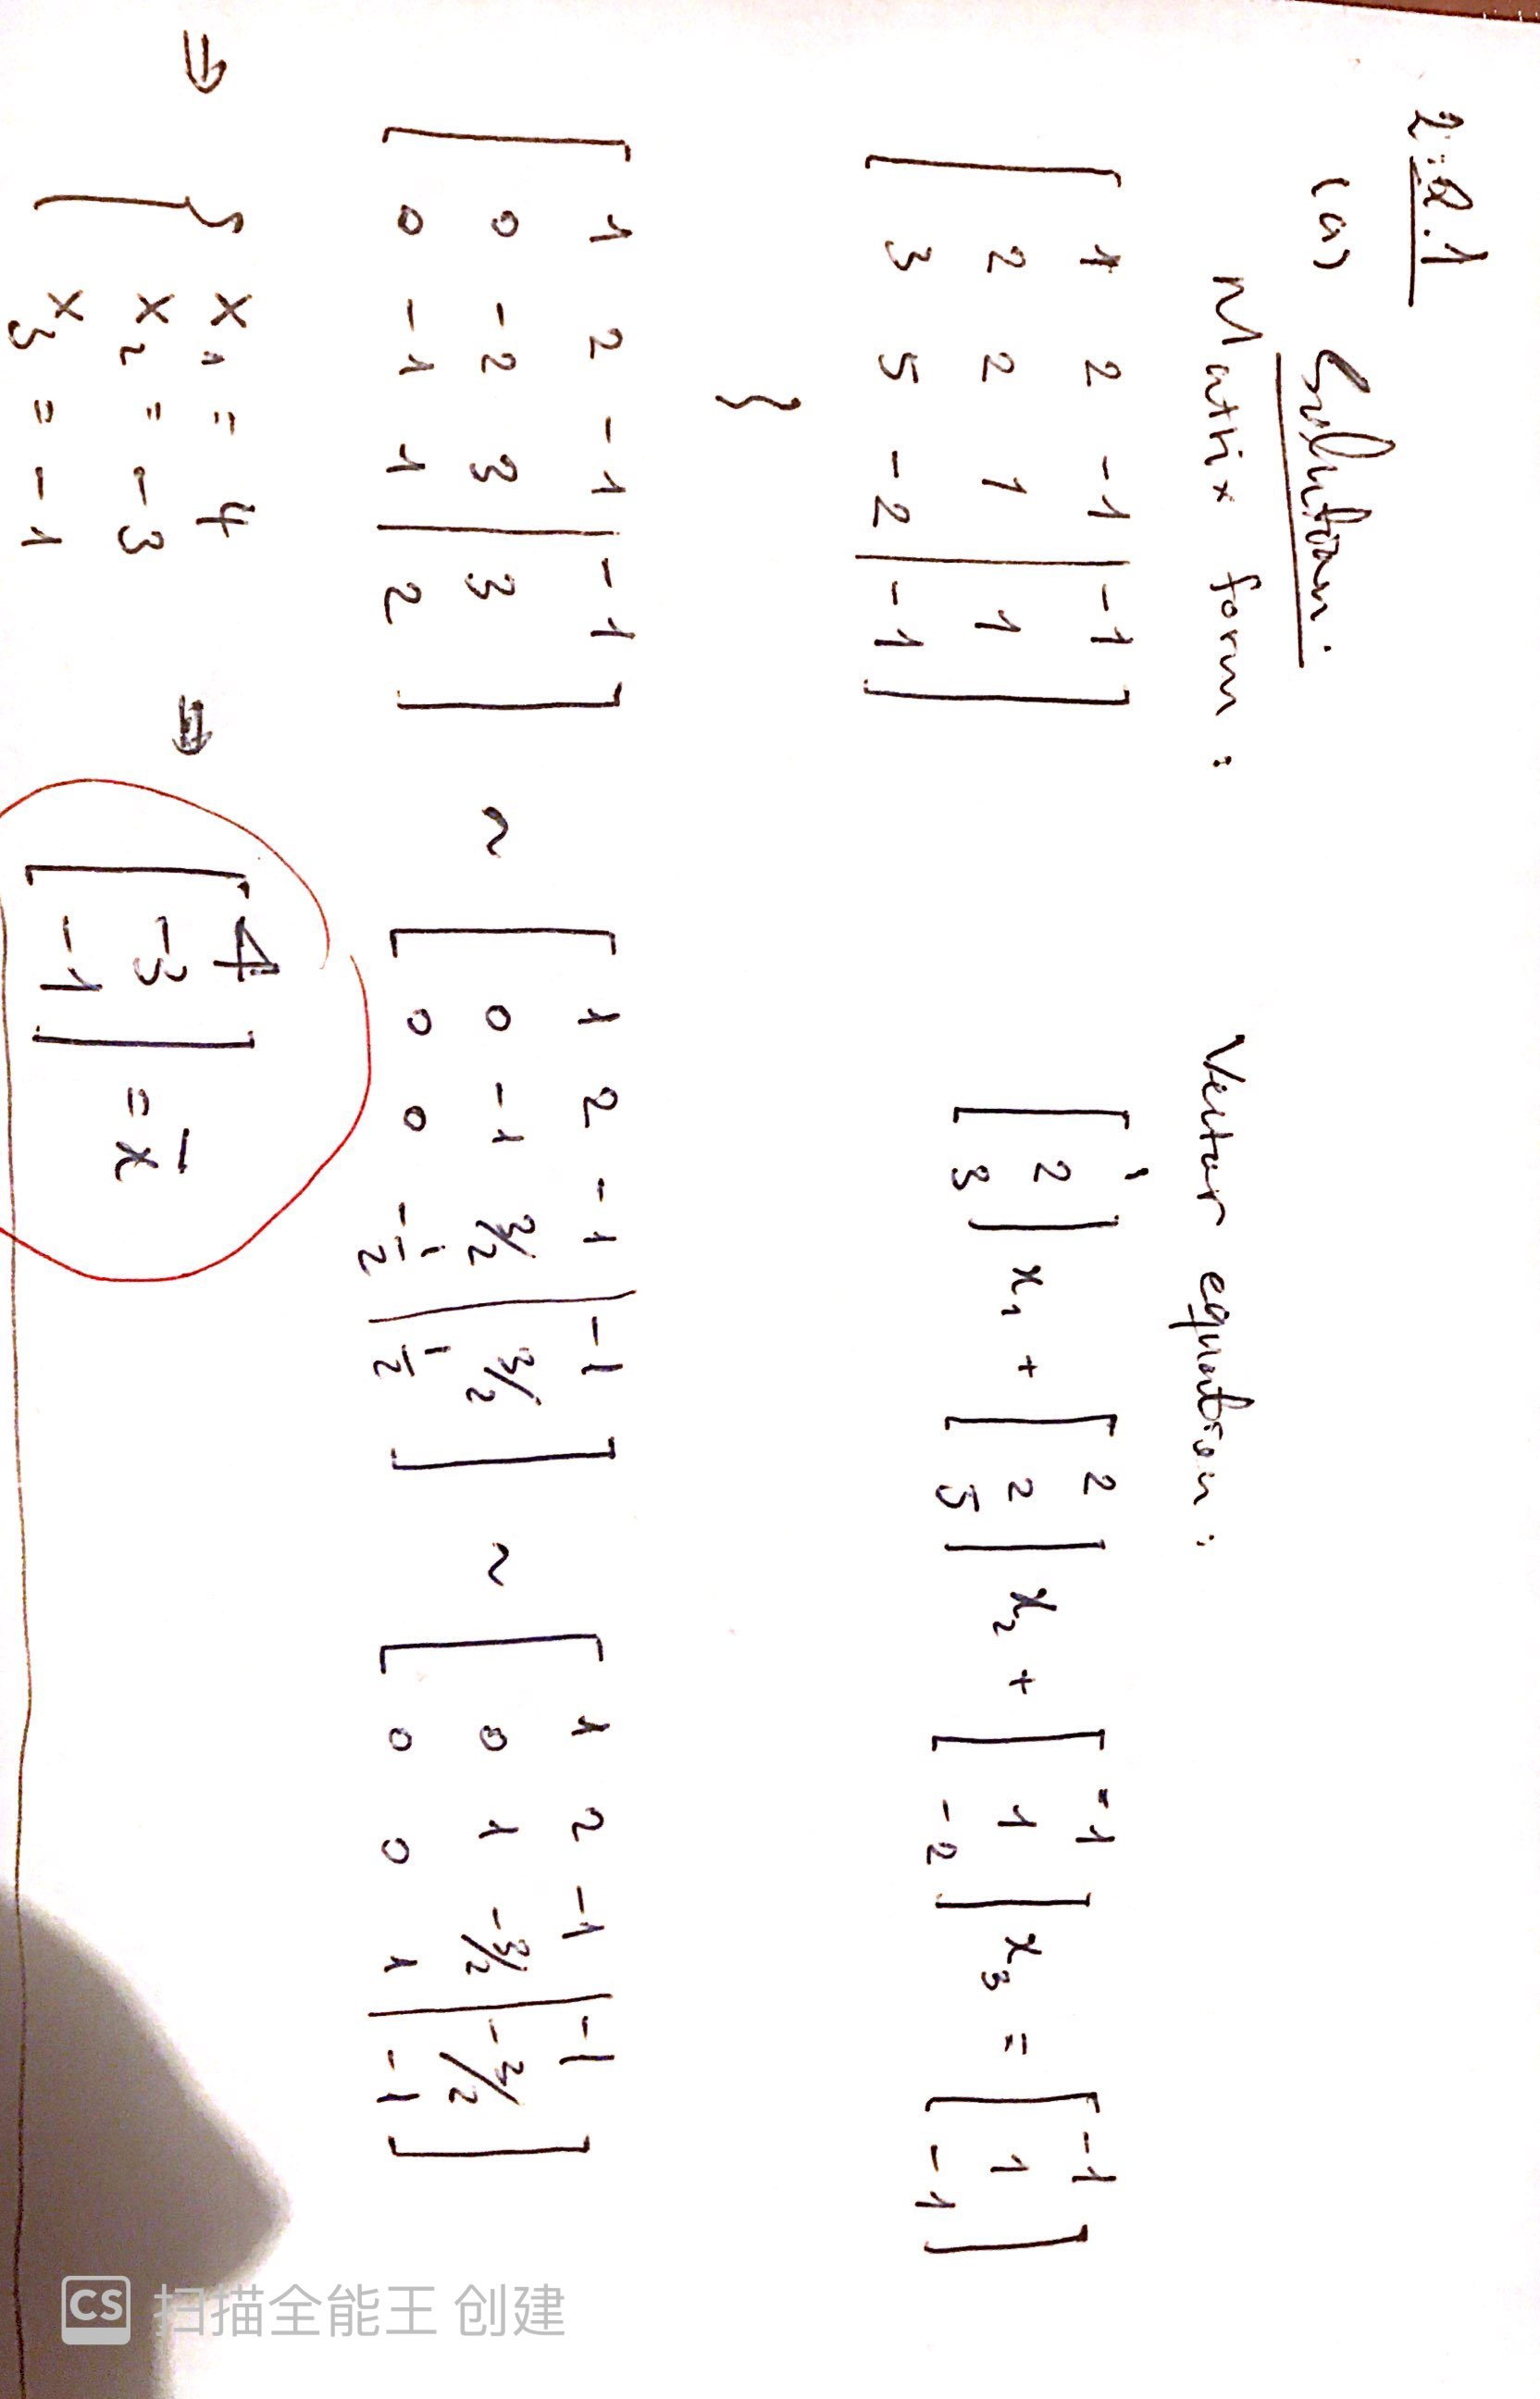
\includegraphics[scale=0.15, angle=90]{images/1a.jpg}\bigbreak
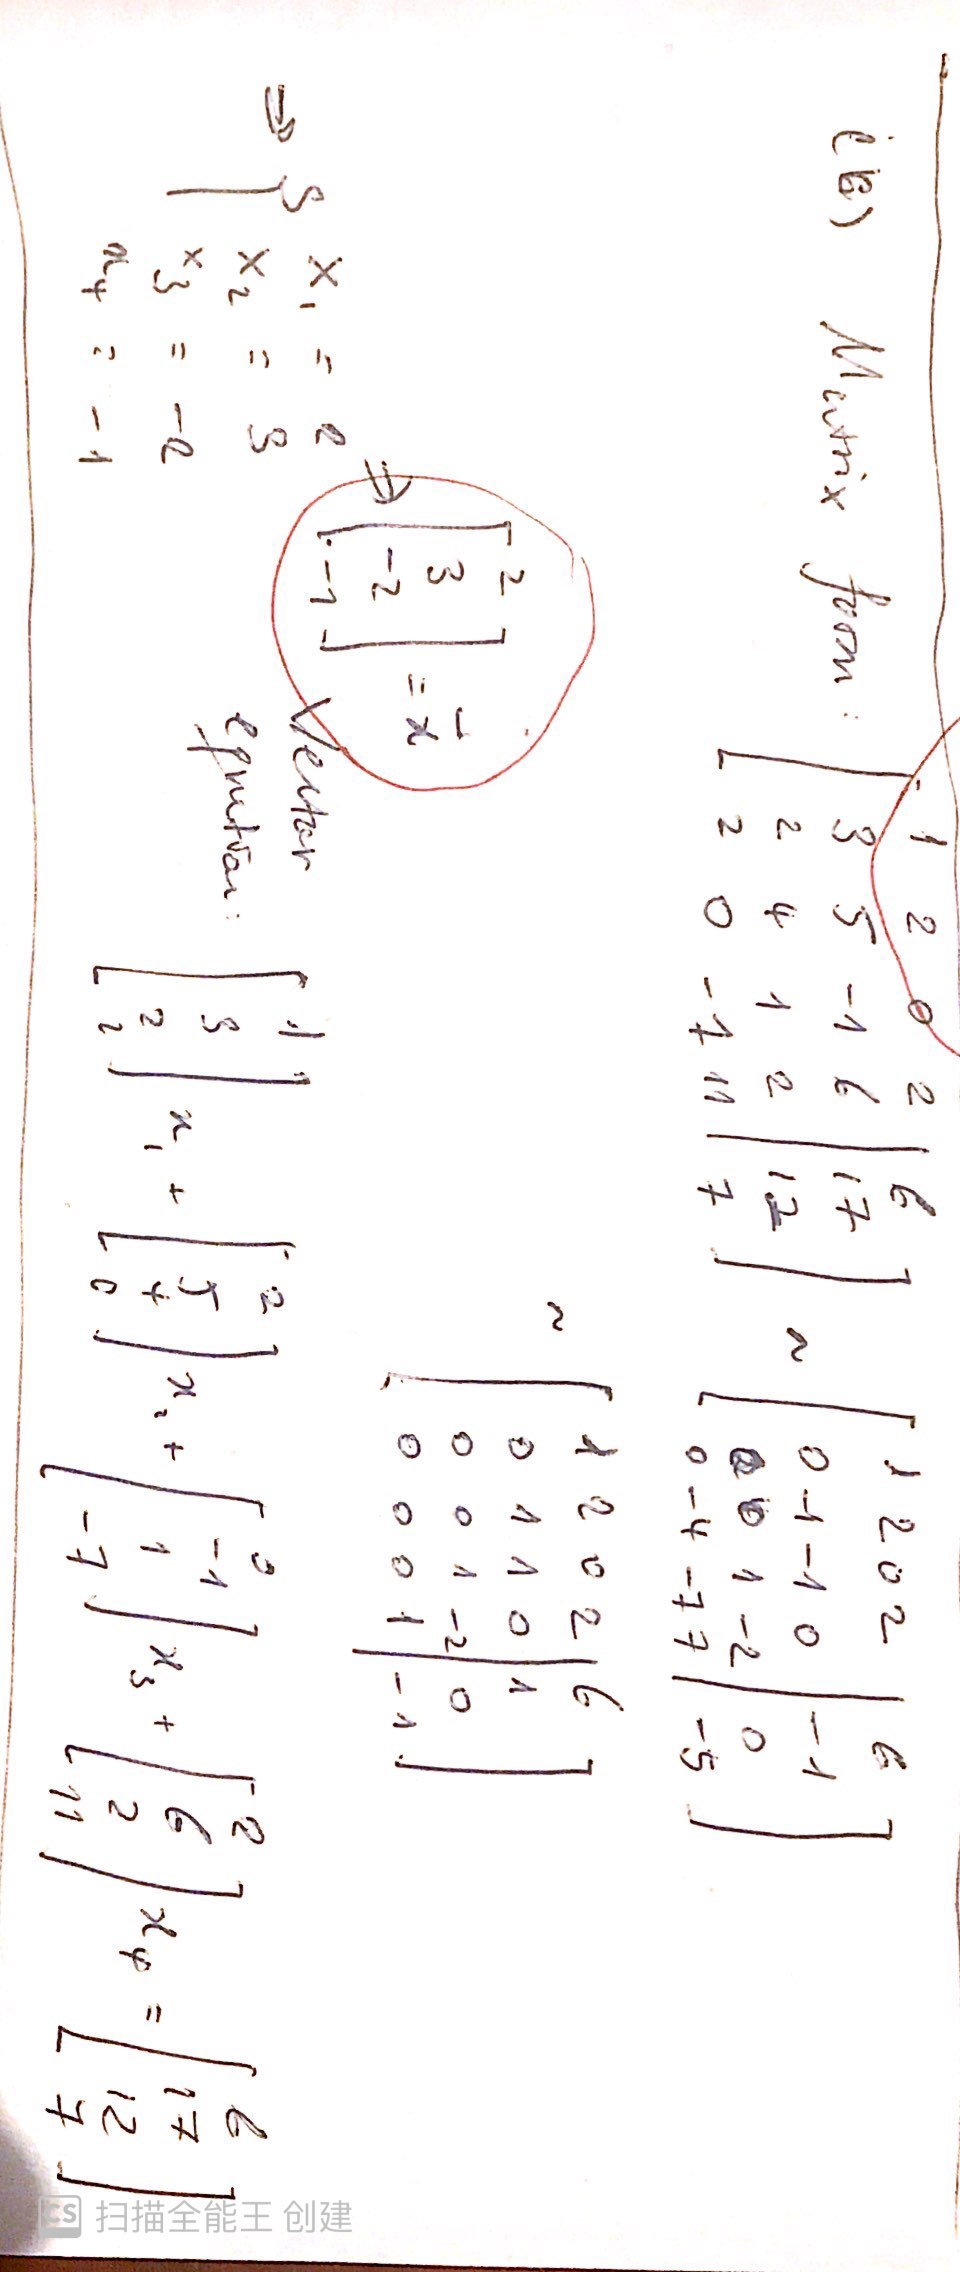
\includegraphics[scale=0.15, angle=90]{images/1b.jpg}\bigbreak
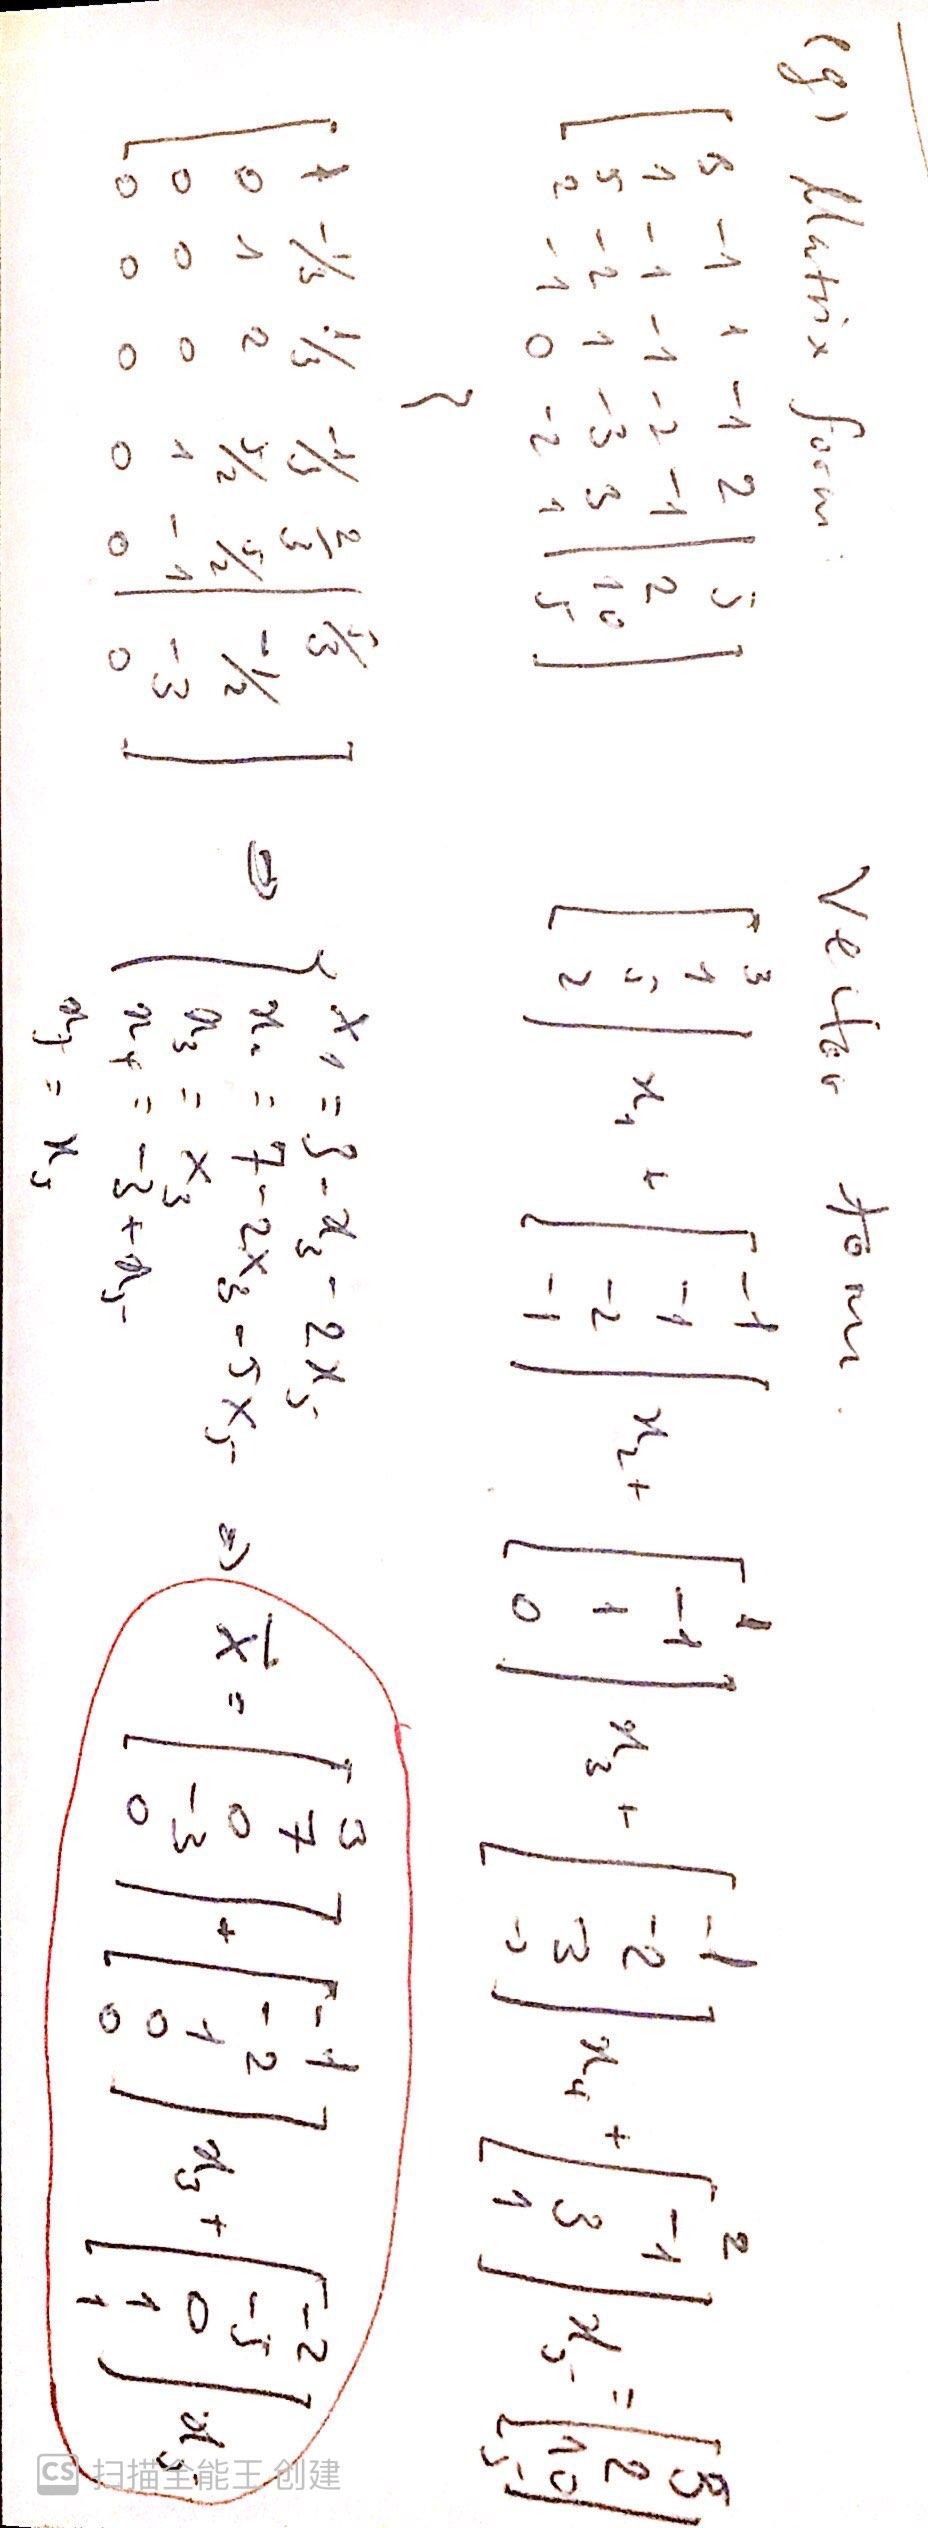
\includegraphics[scale=0.15, angle=90]{images/1c.jpg}
\item (2:2.2) \newline
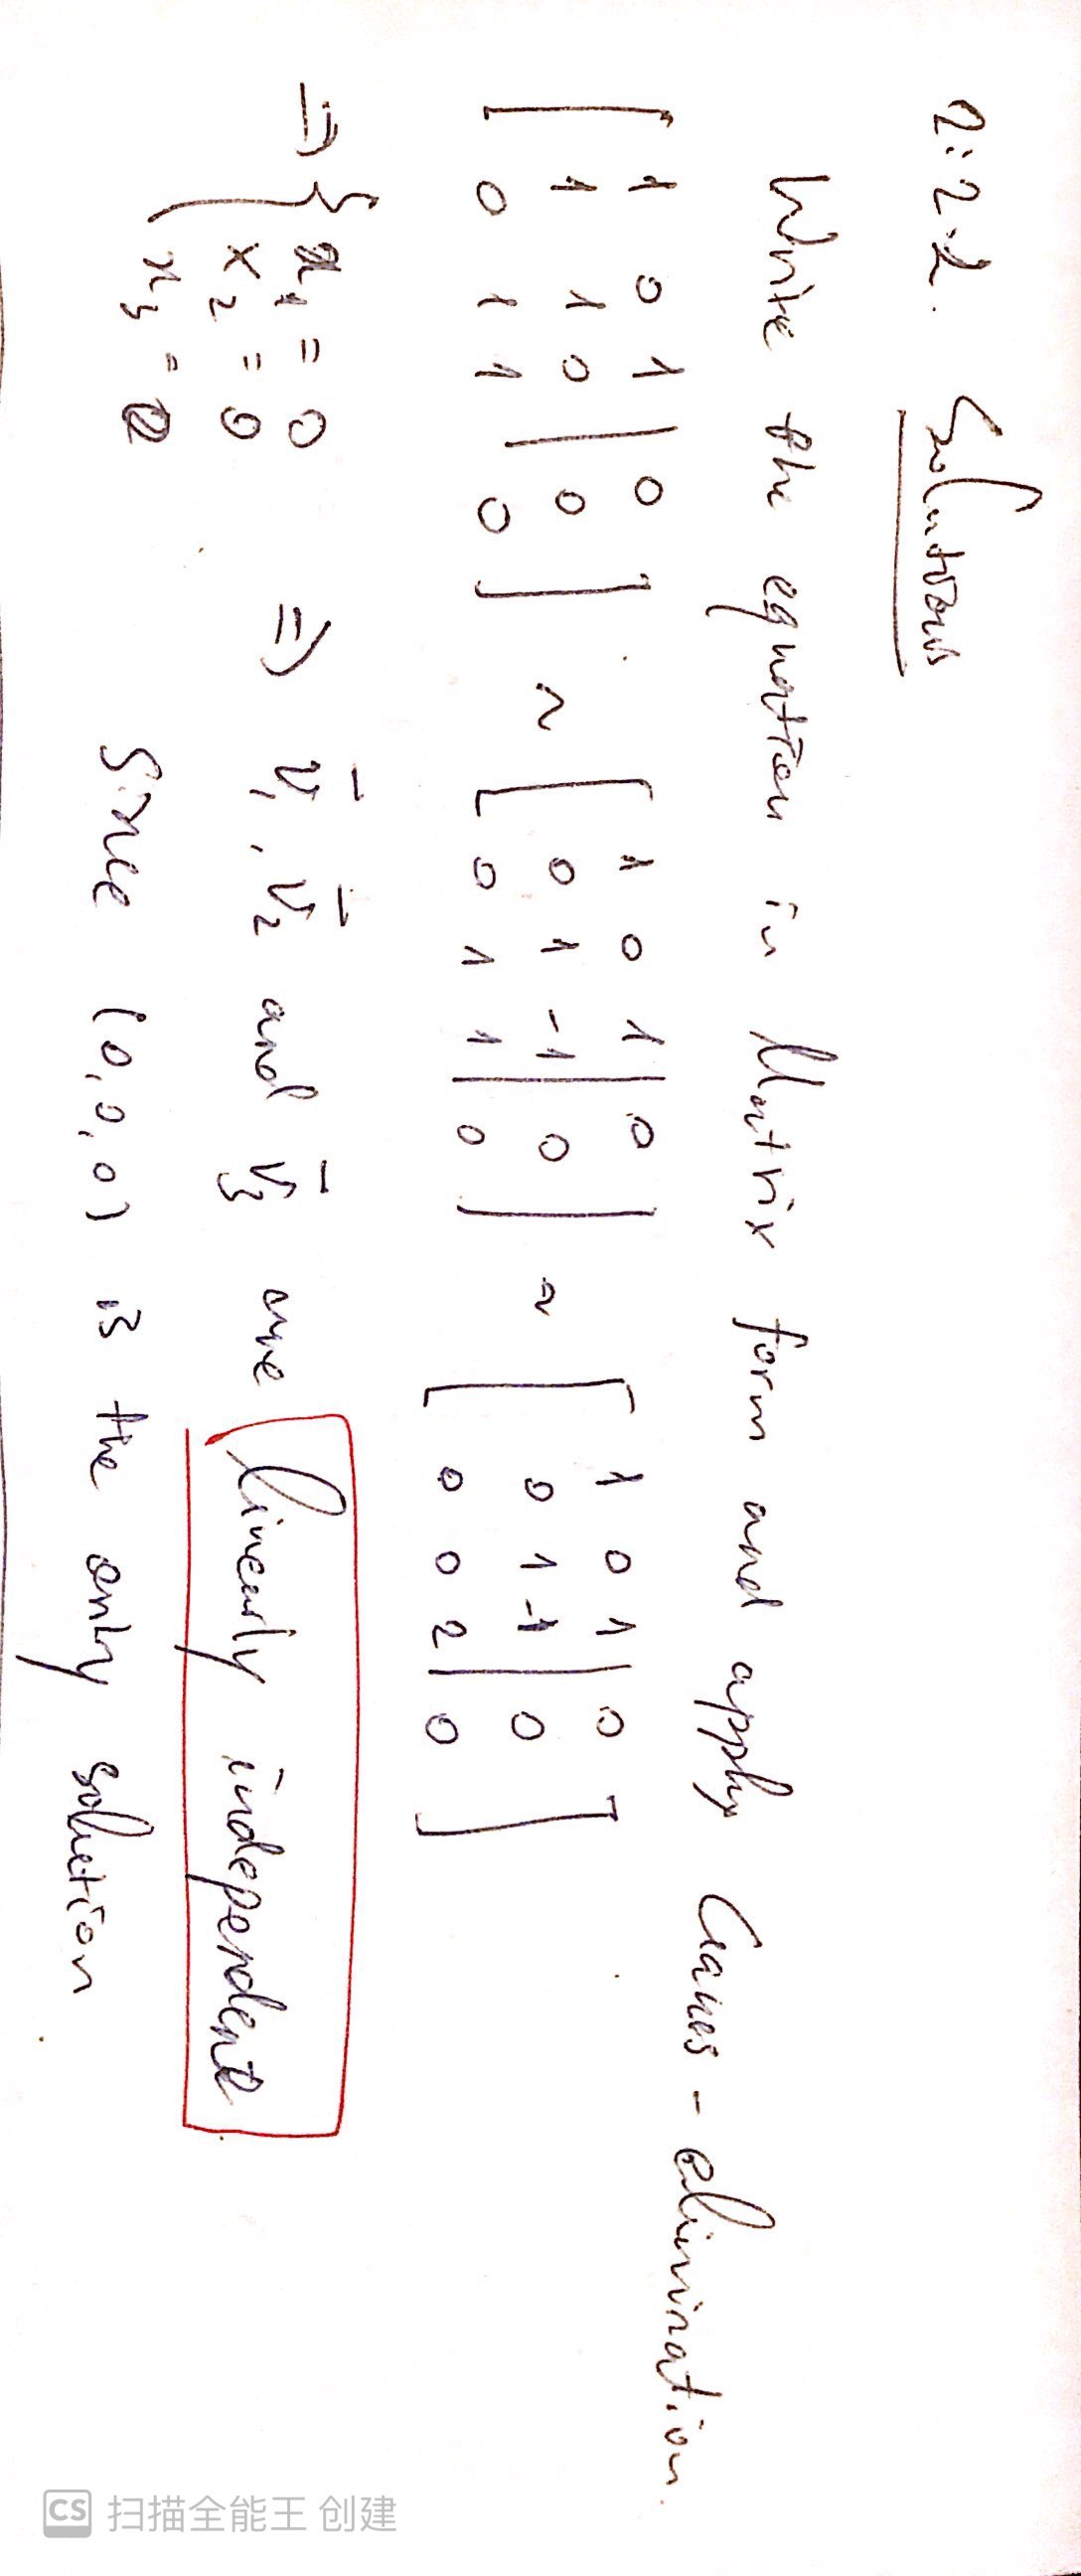
\includegraphics[scale=0.15, angle=90]{images/2.jpg}
\item (2:3.1) \newline
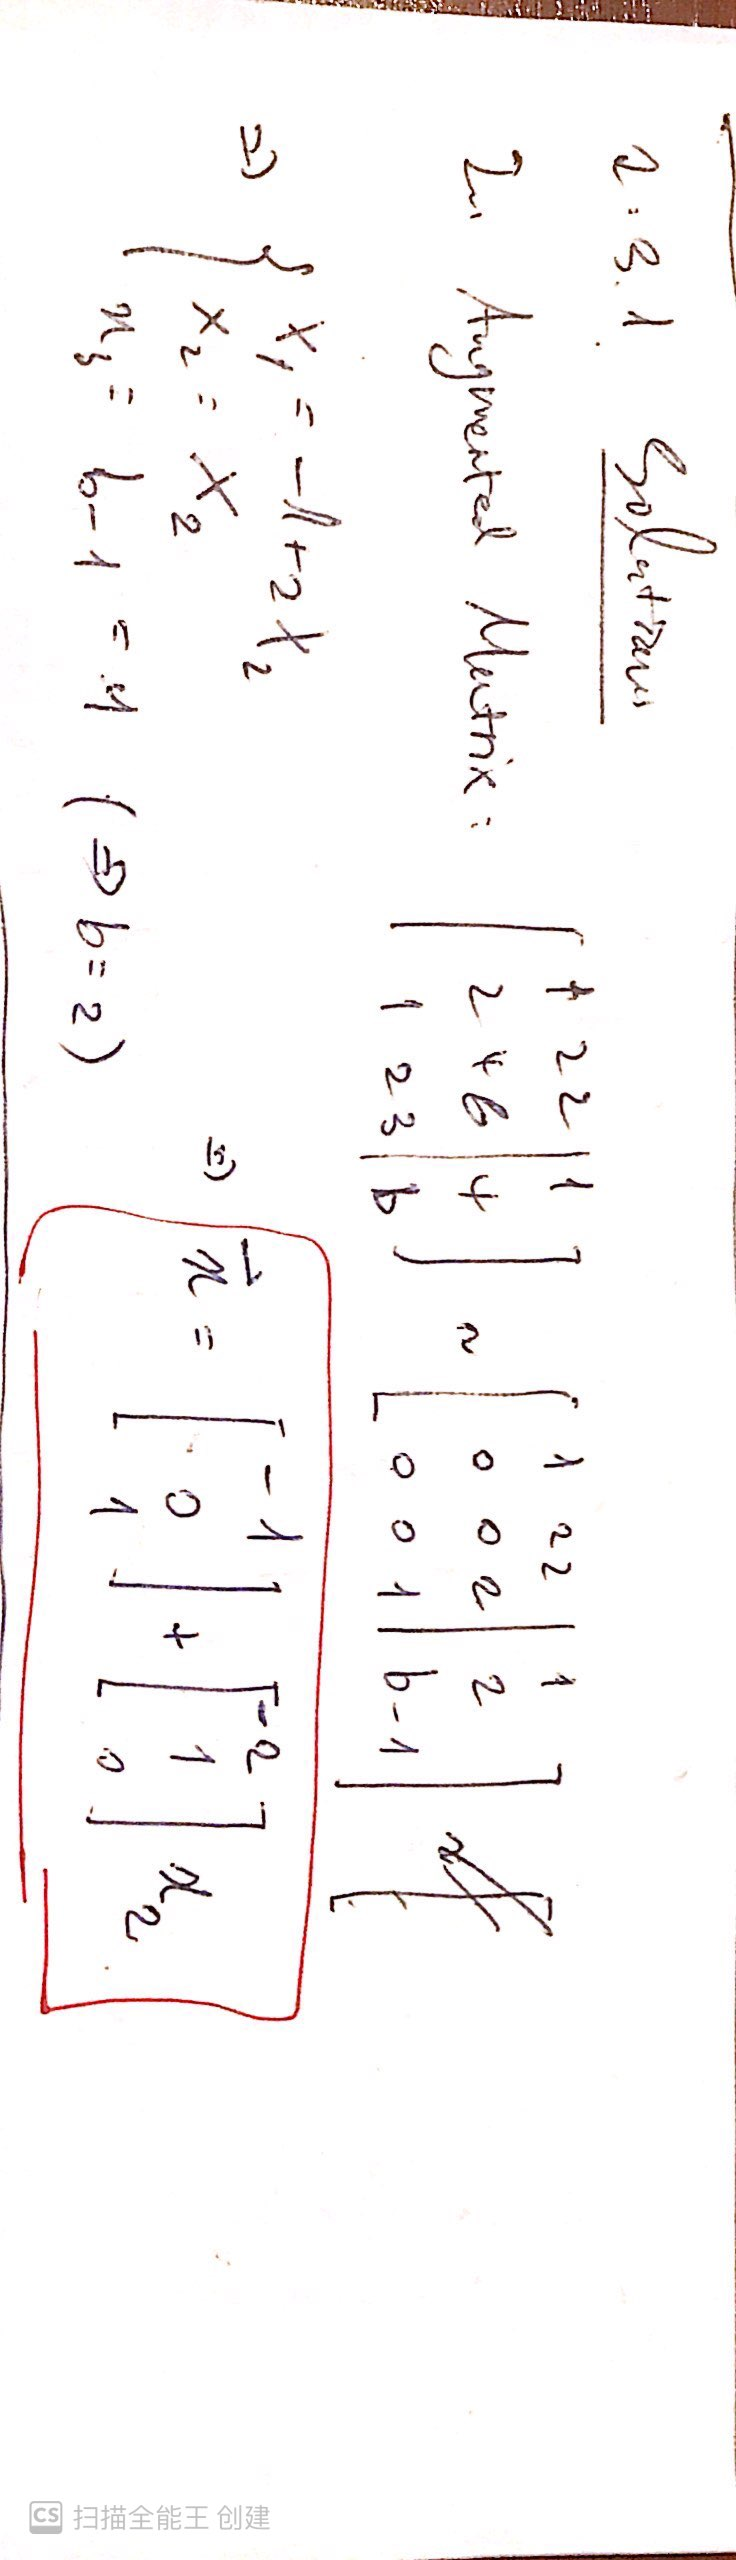
\includegraphics[scale=0.15, angle=90]{images/3.jpg}
\item (2:3.2) \newline
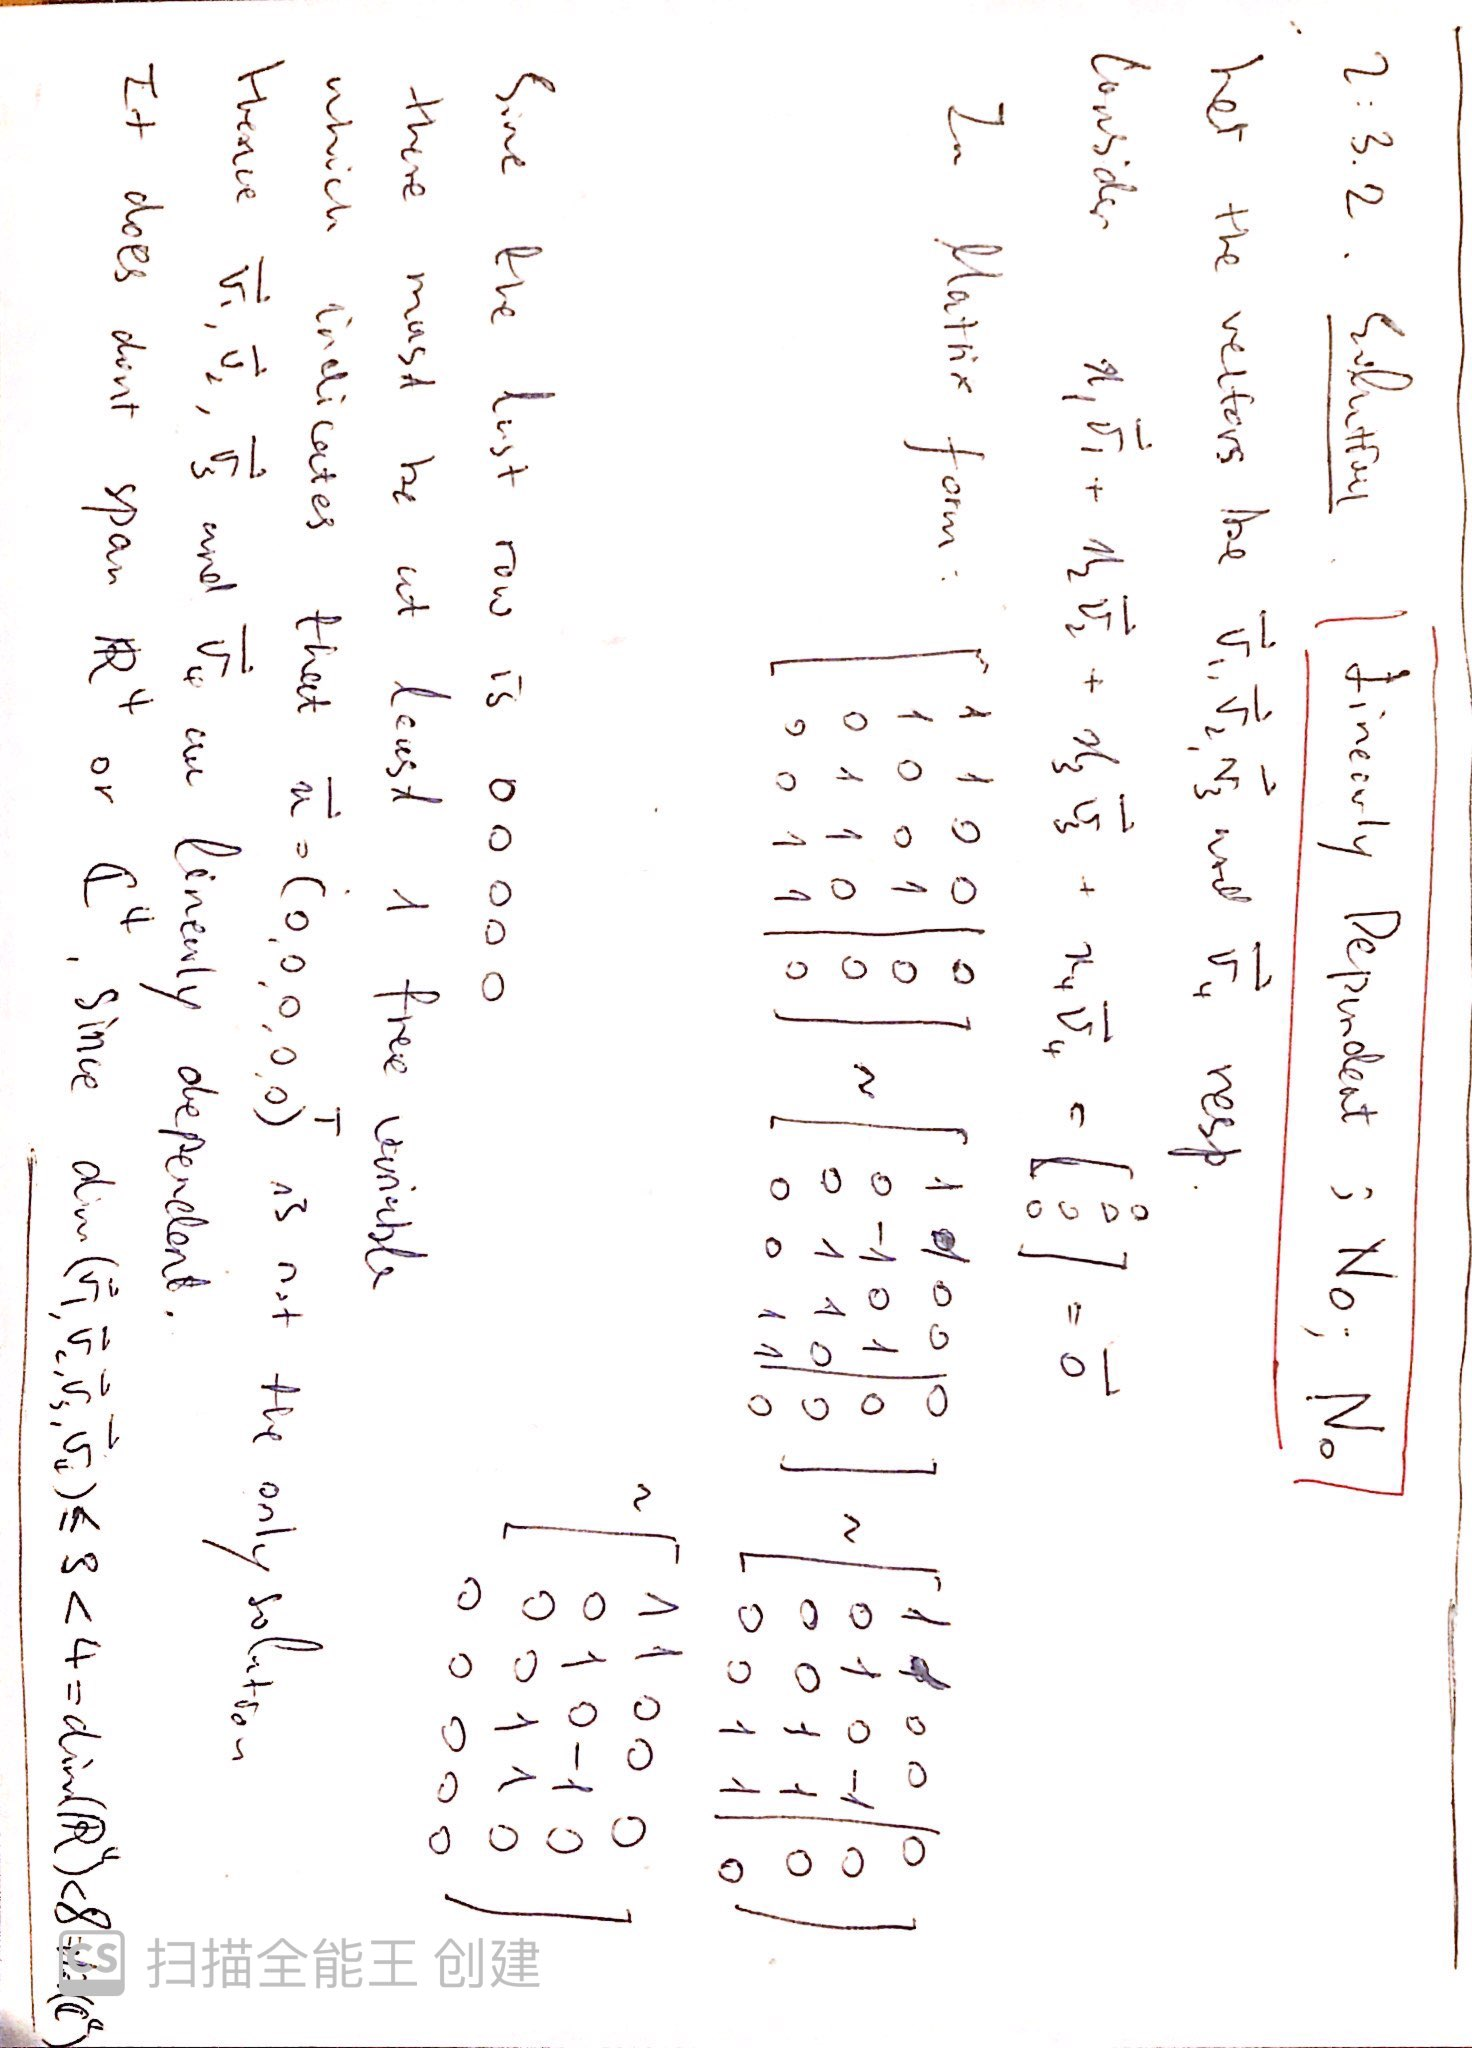
\includegraphics[scale=0.18, angle=90]{images/4.jpg}
\item (2:3.3) (a) \newline
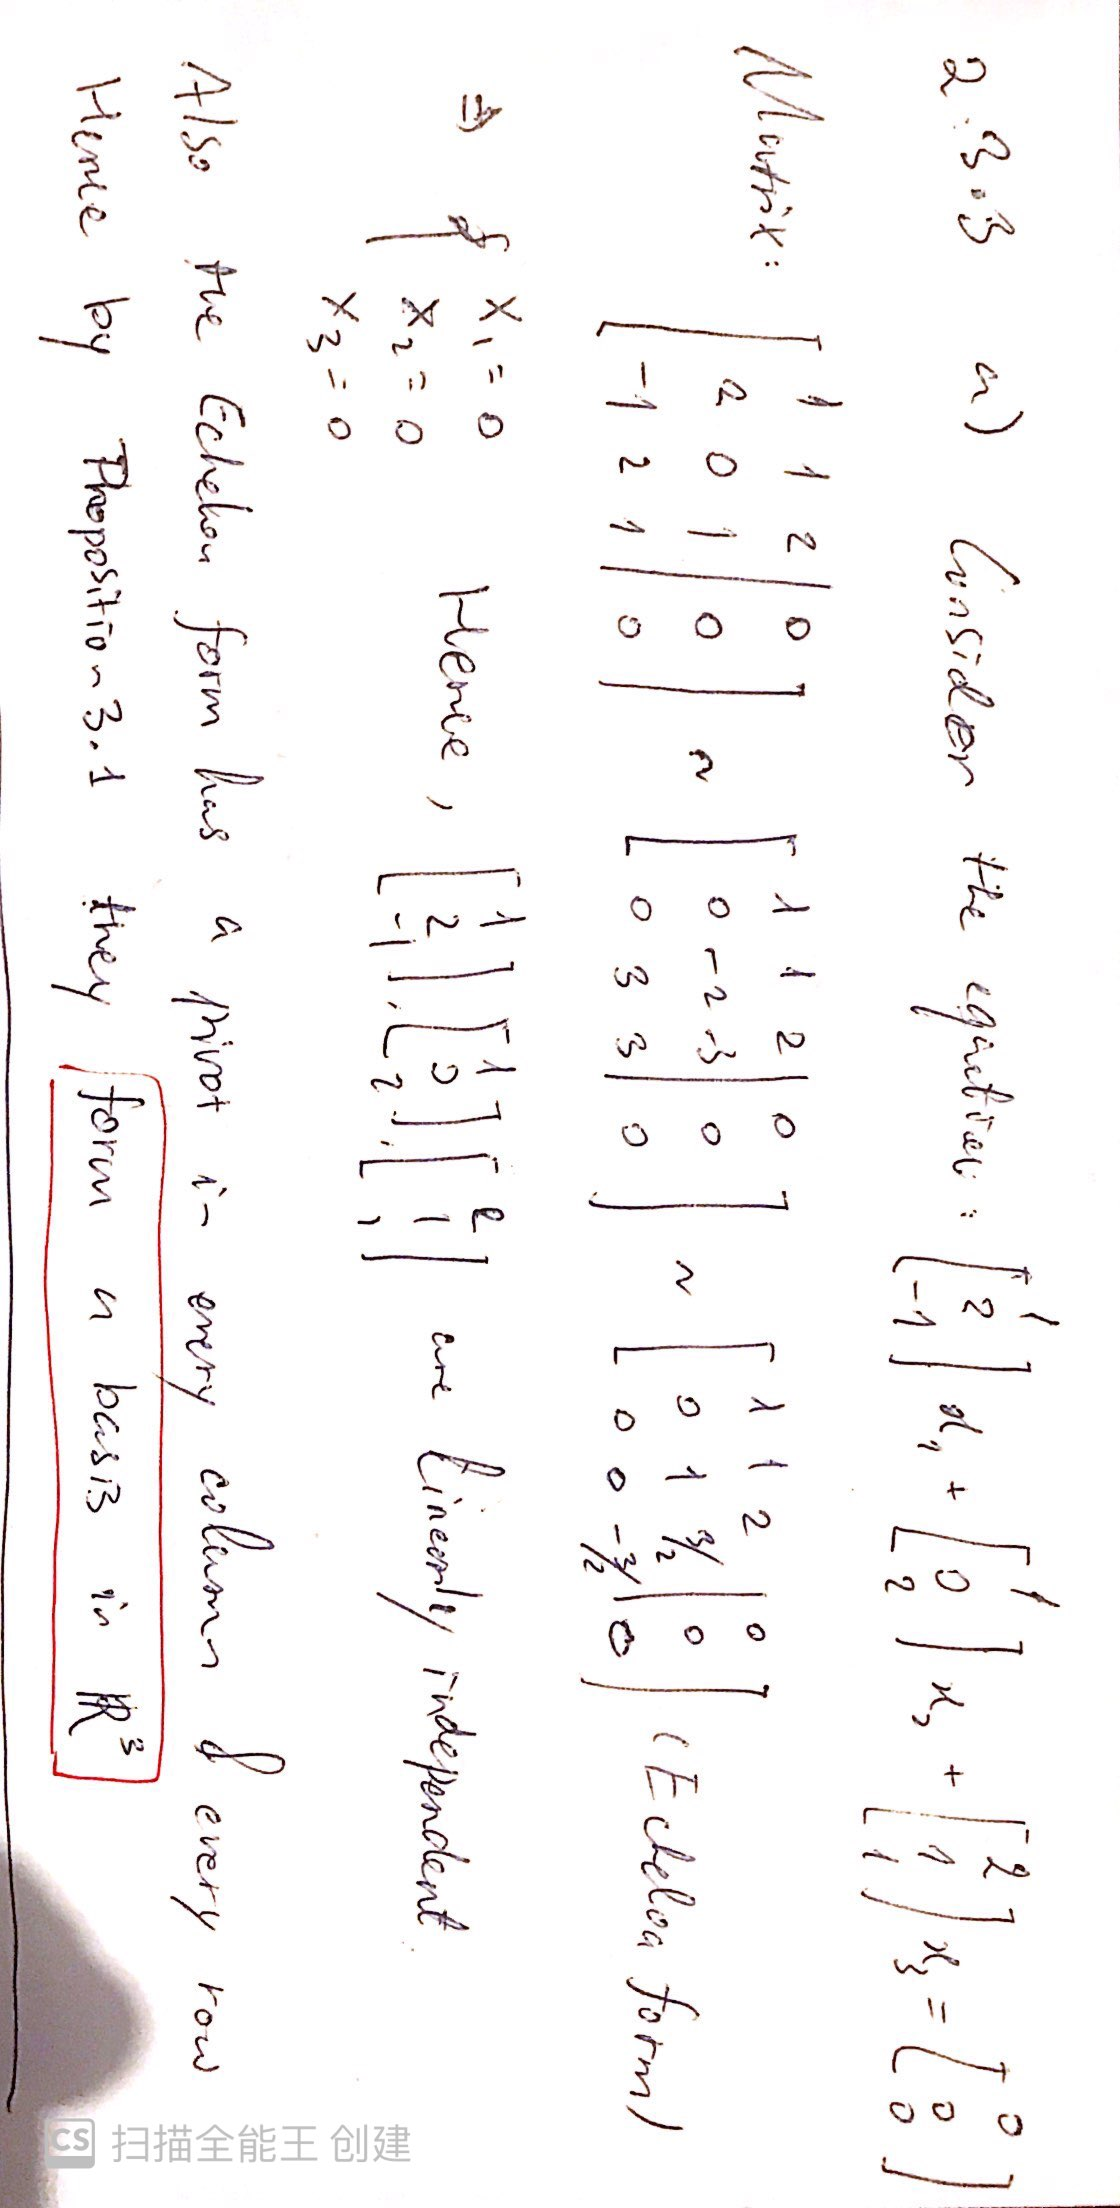
\includegraphics[scale=0.15, angle=90]{images/5.jpg}
\item (2:3.5) \newline
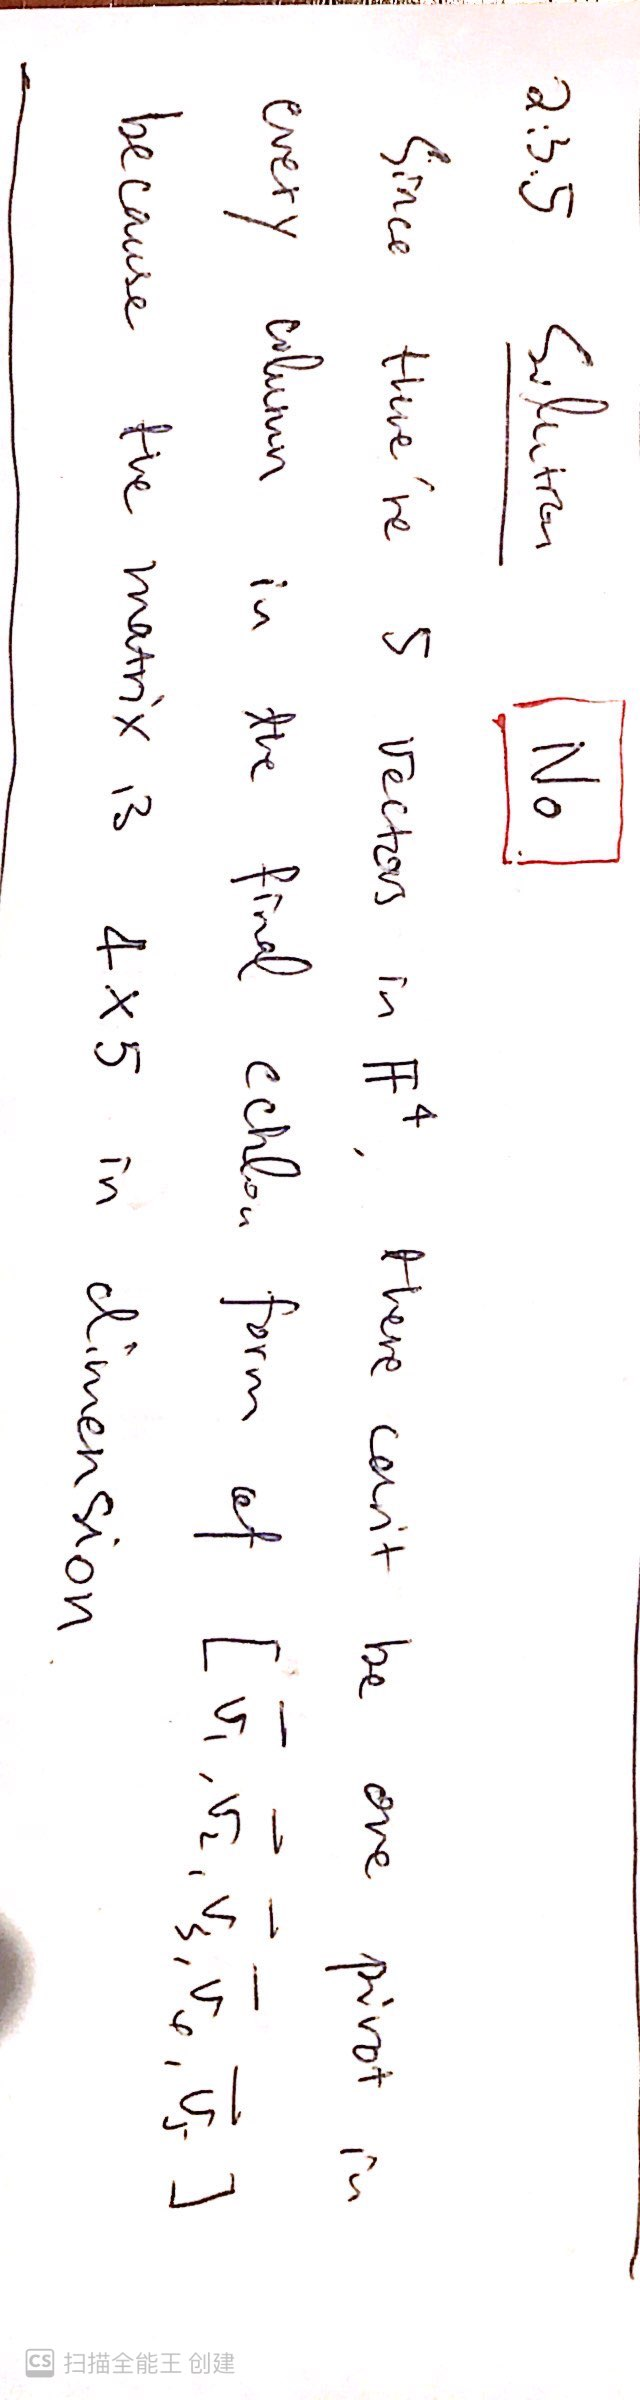
\includegraphics[scale=0.15, angle=90]{images/6.jpg}
\item (2:3.6) \newline
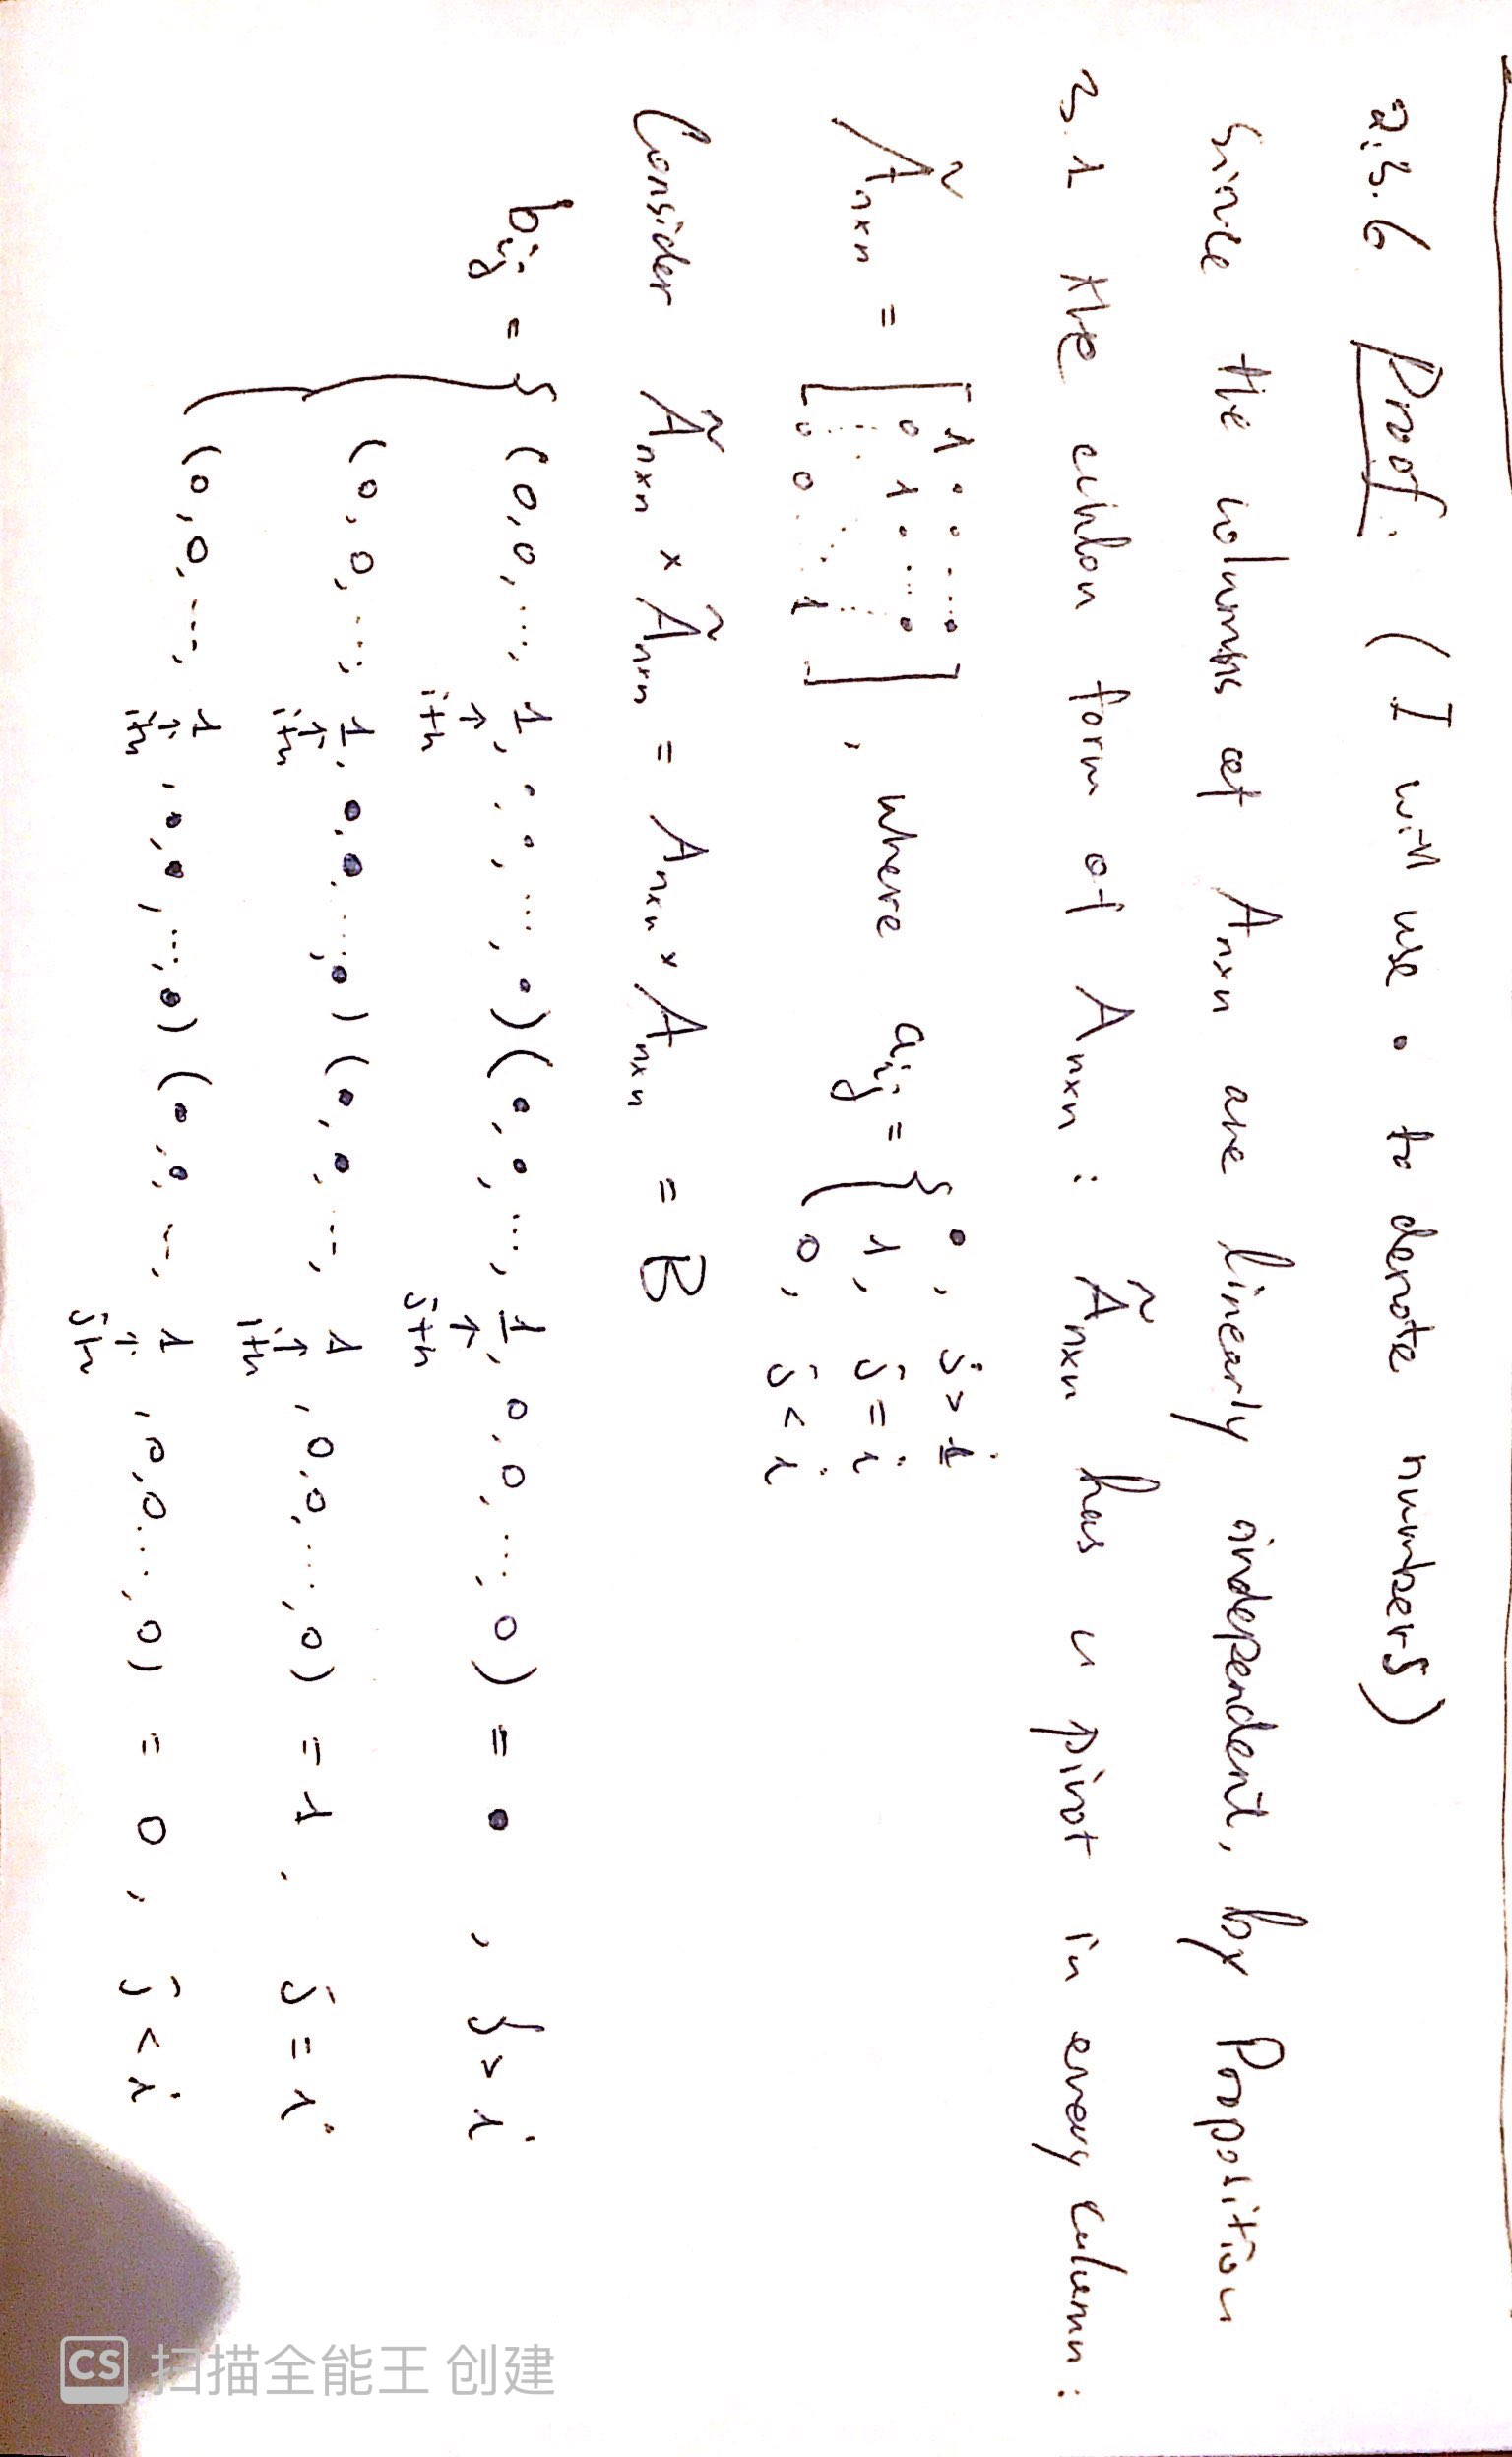
\includegraphics[scale=0.15, angle=90]{images/7.jpg}\newline
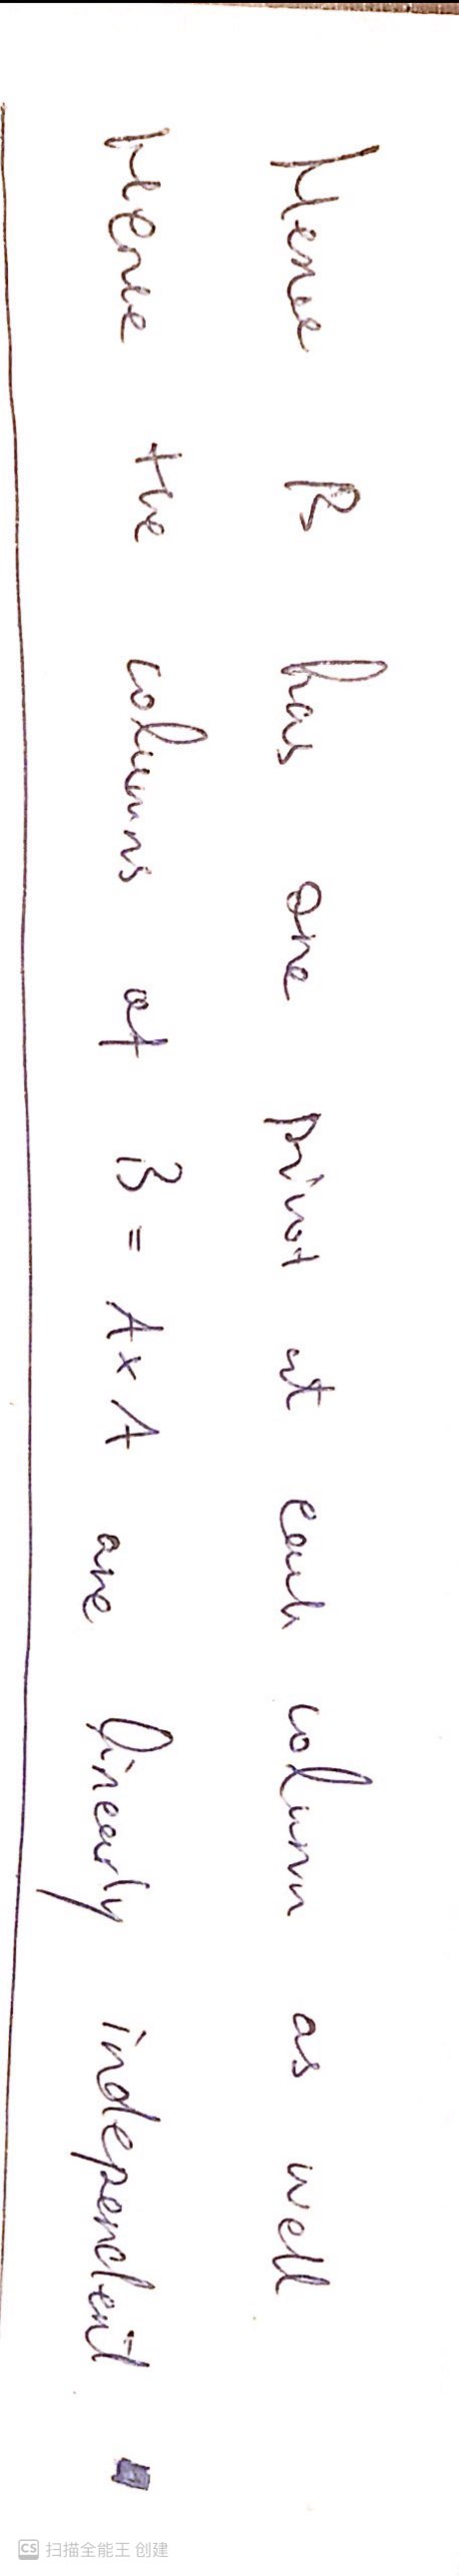
\includegraphics[scale=0.15, angle=90]{images/7b.jpg}
\item (2:3.8) \newline
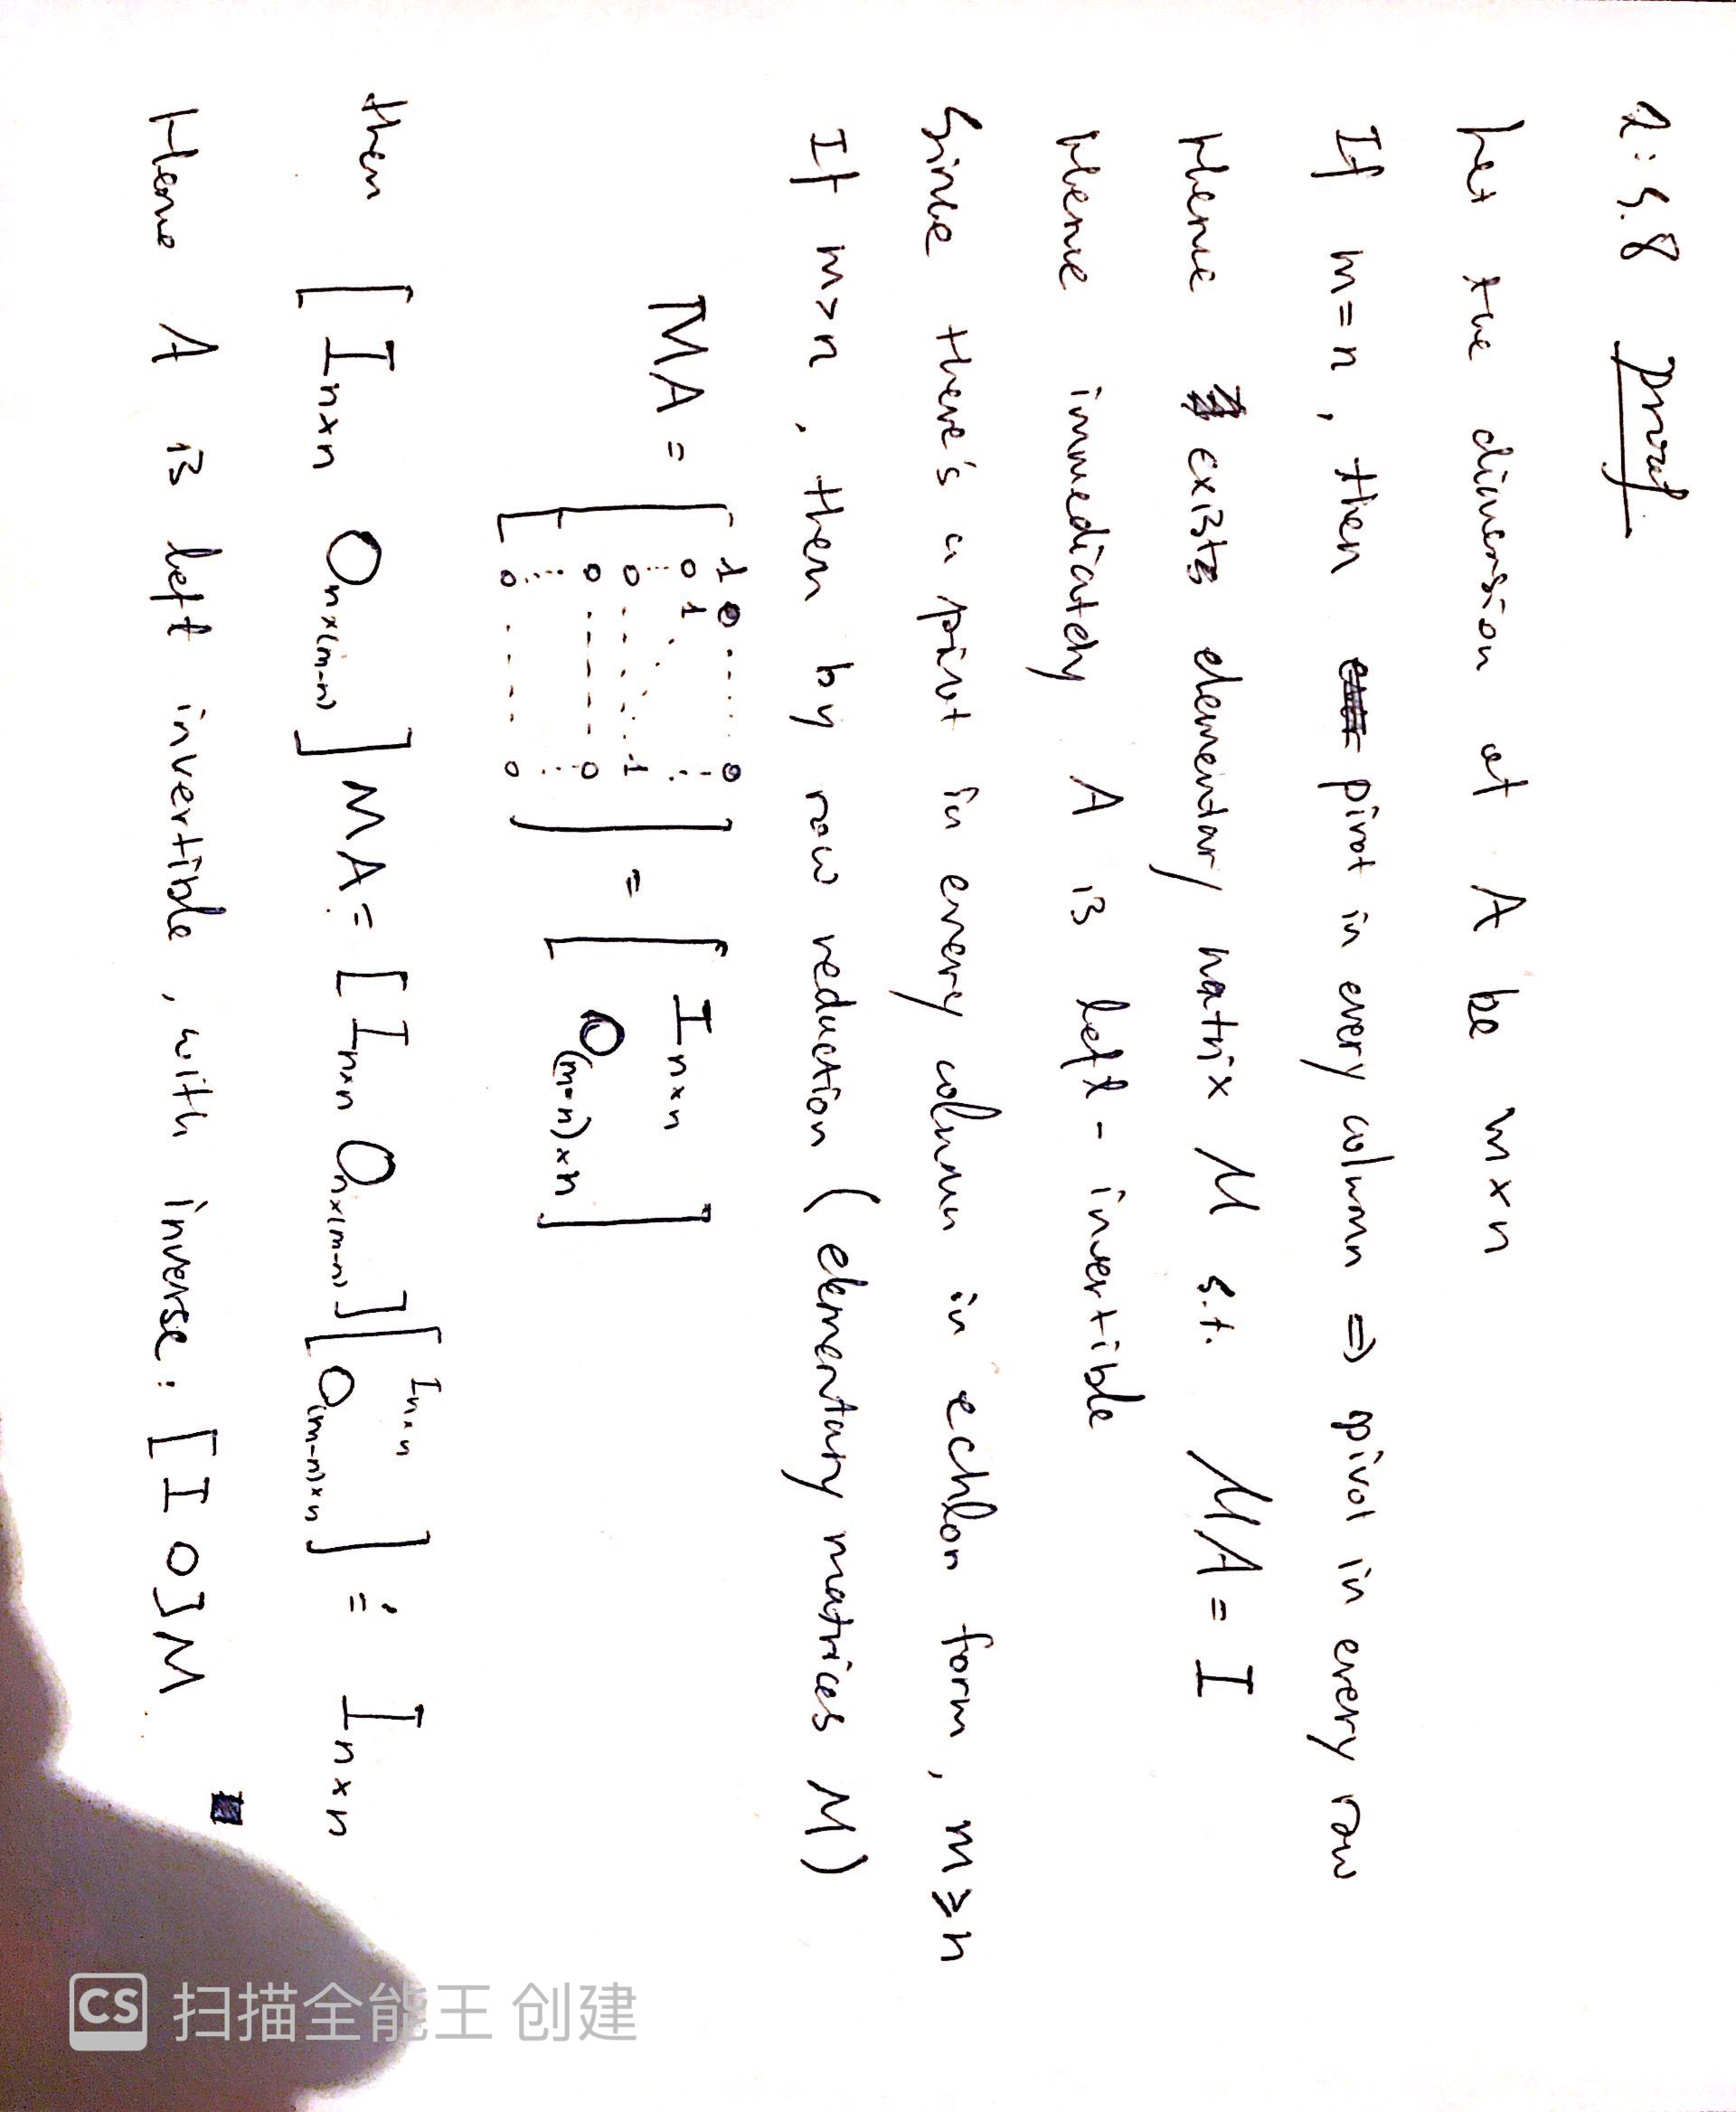
\includegraphics[scale=0.15, angle=90]{images/8.jpg}


\end{enumerate}

\end{document}